\documentclass{ximera}
\graphicspath{  %% When looking for images,
{./}            %% look here first,
{./pictures/}   %% then look for a pictures folder,
{../pictures/}  %% which may be a directory up.
{../../pictures/}  %% which may be a directory up.
{../../../pictures/}  %% which may be a directory up.
{../../../../pictures/}  %% which may be a directory up.
}

\usepackage{listings}
\usepackage{circuitikz}
\usepackage{xcolor}
\usepackage{amsmath,amsthm}
\usepackage{subcaption}
\usepackage{graphicx}
\usepackage{tikz}
\usepackage{tikz-3dplot}
\usepackage{amsfonts}
\usepackage{mdframed} % For framing content
\usepackage{tikz-cd}

  \renewcommand{\vector}[1]{\left\langle #1\right\rangle}
  \newcommand{\arrowvec}[1]{{\overset{\rightharpoonup}{#1}}}
  \newcommand{\ro}{\texttt{R}}%% row operation
  \newcommand{\dotp}{\bullet}%% dot product
  \renewcommand{\l}{\ell}
  \let\defaultAnswerFormat\answerFormatBoxed
  \usetikzlibrary{calc,bending}
  \tikzset{>=stealth}
  




%make a maroon color
\definecolor{maroon}{RGB}{128,0,0}
%make a dark blue color
\definecolor{darkblue}{RGB}{0,0,139}
%define the color fourier0 to be the maroon color
\definecolor{fourier0}{RGB}{128,0,0}
%define the color fourier1 to be the dark blue color
\definecolor{fourier1}{RGB}{0,0,139}
%define the color fourier 1t to be the light blue color
\definecolor{fourier1t}{RGB}{173,216,230}
%define the color fourier2 to be the dark green color
\definecolor{fourier2}{RGB}{0,100,0}
%define teh color fourier2t to be the light green color
\definecolor{fourier2t}{RGB}{144,238,144}
%define the color fourier3 to be the dark purple color
\definecolor{fourier3}{RGB}{128,0,128}
%define the color fourier3t to be the light purple color
\definecolor{fourier3t}{RGB}{221,160,221}
%define the color fourier0t to be the red color
\definecolor{fourier0t}{RGB}{255,0,0}
%define the color fourier4 to be the orange color
\definecolor{fourier4}{RGB}{255,165,0}
%define the color fourier4t to be the darker orange color
\definecolor{fourier4t}{RGB}{255,215,0}
%define the color fourier5 to be the yellow color
\definecolor{fourier5}{RGB}{255,255,0}
%define the color fourier5t to be the darker yellow color
\definecolor{fourier5t}{RGB}{255,255,100}
%define the color fourier6 to be the green color
\definecolor{fourier6}{RGB}{0,128,0}
%define the color fourier6t to be the darker green color
\definecolor{fourier6t}{RGB}{0,255,0}

%New commands for this doc for errors in copying
\newcommand{\eigenvar}{\lambda}
%\newcommand{\vect}[1]{\mathbf{#1}}
\renewcommand{\th}{^{\text{th}}}
\newcommand{\st}{^{\text{st}}}
\newcommand{\nd}{^{\text{nd}}}
\newcommand{\rd}{^{\text{rd}}}
\newcommand{\paren}[1]{\left(#1\right)}
\newcommand{\abs}[1]{\left|#1\right|}
\newcommand{\R}{\mathbb{R}}
\newcommand{\C}{\mathbb{C}}
\newcommand{\Hilb}{\mathbb{H}}
\newcommand{\qq}[1]{\text{#1}}
\newcommand{\Z}{\mathbb{Z}}
\newcommand{\N}{\mathbb{N}}
\newcommand{\q}[1]{\text{``#1''}}
%\newcommand{\mat}[1]{\begin{bmatrix}#1\end{bmatrix}}
\newcommand{\rref}{\text{reduced row echelon form}}
\newcommand{\ef}{\text{echelon form}}
\newcommand{\ohm}{\Omega}
\newcommand{\volt}{\text{V}}
\newcommand{\amp}{\text{A}}
\newcommand{\Seq}{\textbf{Seq}}
\newcommand{\Poly}{\textbf{P}}
\renewcommand{\quad}{\text{    }}
\newcommand{\roweq}{\simeq}
\newcommand{\rowop}{\simeq}
\newcommand{\rowswap}{\leftrightarrow}
\newcommand{\Mat}{\textbf{M}}
\newcommand{\Func}{\textbf{Func}}
\newcommand{\Hw}{\textbf{Hamming weight}}
\newcommand{\Hd}{\textbf{Hamming distance}}
\newcommand{\rank}{\text{rank}}
\newcommand{\longvect}[1]{\overrightarrow{#1}}
% Define the circled command
\newcommand{\circled}[1]{%
  \tikz[baseline=(char.base)]{
    \node[shape=circle,draw,inner sep=2pt,red,fill=red!20,text=black] (char) {#1};}%
}

% Define custom command \strikeh that just puts red text on the 2nd argument
\newcommand{\strikeh}[2]{\textcolor{red}{#2}}

% Define custom command \strikev that just puts red text on the 2nd argument
\newcommand{\strikev}[2]{\textcolor{red}{#2}}

%more new commands for this doc for errors in copying
\newcommand{\SI}{\text{SI}}
\newcommand{\kg}{\text{kg}}
\newcommand{\m}{\text{m}}
\newcommand{\s}{\text{s}}
\newcommand{\norm}[1]{\left\|#1\right\|}
\newcommand{\col}{\text{col}}
\newcommand{\sspan}{\text{span}}
\newcommand{\proj}{\text{proj}}
\newcommand{\set}[1]{\left\{#1\right\}}
\newcommand{\degC}{^\circ\text{C}}
\newcommand{\centroid}[1]{\overline{#1}}
\newcommand{\dotprod}{\boldsymbol{\cdot}}
%\newcommand{\coord}[1]{\begin{bmatrix}#1\end{bmatrix}}
\newcommand{\iprod}[1]{\langle #1 \rangle}
\newcommand{\adjoint}{^{*}}
\newcommand{\conjugate}[1]{\overline{#1}}
\newcommand{\eigenvarA}{\lambda}
\newcommand{\eigenvarB}{\mu}
\newcommand{\orth}{\perp}
\newcommand{\bigbracket}[1]{\left[#1\right]}
\newcommand{\textiff}{\text{ if and only if }}
\newcommand{\adj}{\text{adj}}
\newcommand{\ijth}{\emph{ij}^\text{th}}
\newcommand{\minor}[2]{M_{#2}}
\newcommand{\cofactor}{\text{C}}
\newcommand{\shift}{\textbf{shift}}
\newcommand{\startmat}[1]{
  \left[\begin{array}{#1}
}
\newcommand{\stopmat}{\end{array}\right]}
%a command to give a name to explorations and hints and theorems
\newcommand{\name}[1]{\begin{centering}\textbf{#1}\end{centering}}
\newcommand{\vect}[1]{\vec{#1}}
\newcommand{\dfn}[1]{\textbf{#1}}
\newcommand{\transpose}{\mathsf{T}}
\newcommand{\mtlb}[2][black]{\texttt{\textcolor{#1}{#2}}}
\newcommand{\RR}{\mathbb{R}} % Real numbers
\newcommand{\id}{\text{id}}


%Some boiler plate for putting matlab in 
%Write A as a matrix in MATLAB in a lstlisting environment
%\begin{lstlisting}[style=Matlab]
%    A = [1 0 3; 0 1 5; 1 1 8]
%    reduced=rref(A)
%\end{lstlisting}

\author{Zack Reed}
%borrowed from selinger linear algebra
\title{Chapter Two Mini-Project: Image Manipulation}
\begin{document}
\begin{abstract}

    This is a mini-project walking you through image manipulation with matrices. Exposure to this code will help you prepare for the final project.

\end{abstract}
\maketitle


\section*{Smiley Faces}

\begin{problem}
{\bf - Smiley Face Manipulation}

First, load the smiley matrix and display it so that you can see the matrix and its values.
\begin{verbatim}
load linalg/smiley.mat
smiley
\end{verbatim}

\begin{enumerate}

\item Now, use the provided function ``\texttt{smiley\_show}" from the course helper functions to visualize the smiley face as a figure.

\begin{verbatim}
linalg.smiley_show(smiley)
\end{verbatim}

You should see the following 21x21 image:
%include a centered image of the smiley face
\begin{center}
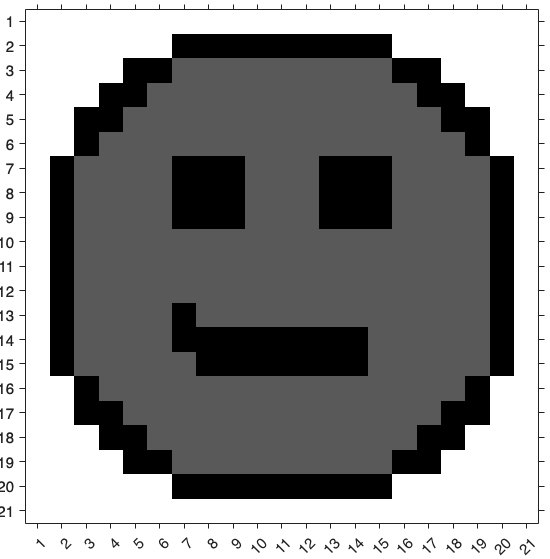
\includegraphics[width=0.6\textwidth]{smiley_base.png}
\end{center}

\item Now change the smiley's right eye (on your left) to a wink, aka a diagonal of black, filling in the blanks of the code as your final answer.
\begin{hint}
First copy the code into MATLAB to try things, or use the provided course live script, rather than guessing in this assignment first.
\end{hint}

First, make a $3\times 3$ grid to replace the right eye. We'll at first make it all 100 so that it's the face color, then fill in the diagonal with 0 (black). The $\texttt{ones}$ function makes a matrix of all 1s, of the dimension you specify.
\begin{verbatim}
right_wink=100*ones(3,3);
\end{verbatim}

Make a copy of the smiley face so you preserve the original.
\begin{verbatim}
smiley_wink=smiley;
\end{verbatim}

Now fill in the diagonal of the wink matrix with black.

\mtlb[blue]{for }\mtlb{ i=1:3} \\
\mtlb{\hspace{1cm}right\_wink(}$\answer[format=string]{i}$,$\answer[format=string]{i}$)=$\answer{0};$\\
\mtlb[blue]{end}

Now replace the eye on the smiley face with the wink.
\begin{hint}
The right eye is located on rows 7-9 columns 7-9 of the smiley face matrix.
\end{hint}

\mtlb{smiley\_wink(}$\answer{7}$:$\answer{9}$,$\answer{7}$:$\answer{9}$\mtlb{)=right\_wink};

View the results to check you replaced the eye correctly.
\begin{verbatim}
linalg.smiley_show(smiley_wink)
\end{verbatim}

It should look like this:
%include a centered image of the wink
\begin{center}
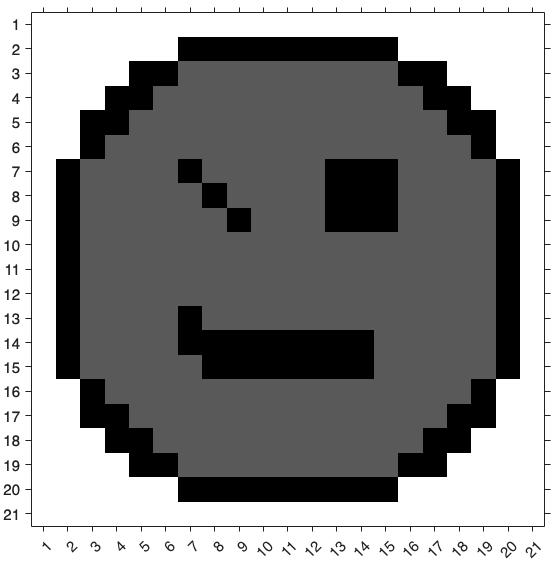
\includegraphics[width=0.6\textwidth]{smiley_wink.png}
\end{center}

\item Now we want to swap which eye is winking, which will involve rotating the wink pixels. To do this, we'll want to multiply right\_wink by a matrix that swaps the first and third column vectors. 

To figure out the swapping matrix, think about where you'd send $i$, $j$, and $k$ if you wanted your linear transformation to swap the positions of $i$ and $k$, but leave $j$ where it is.

\mtlb{wink\_rotated=}[$\answer{0}$, $\answer{0}$, $\answer{1}$; $\answer{0}$, $\answer{1}$, $\answer{0}$; $\answer{1}$, $\answer{0}$, $\answer{0}$]*\mtlb{right\_wink};

Now fill in the right eye using the left eye, located in rows 7-9 columns 13-15.

\mtlb{smiley\_wink(}$\answer{7}$:$\answer{9}$,$\answer{7}$:$\answer{9}$\mtlb{)=smiley\_wink(}$\answer{7}$:$\answer{9}$,$\answer{13}$:$\answer{15}$\mtlb{)};

Now fill in the left eye with the new wink.

\mtlb{smiley\_wink(}$\answer{7}$:$\answer{9}$,$\answer{13}$:$\answer{15}$\mtlb{)=}$\answer[format=string]{wink\_rotated}$\mtlb{;}

Finally, view the result to check your work. If you mess up, you'll want to re-do the cell creating the right-eye wink to reset the matrix smiley\_wink.
\begin{verbatim}
linalg.smiley_show(smiley_wink)
\end{verbatim}

It should look like this:
%include a centered image of the wink
\begin{center}
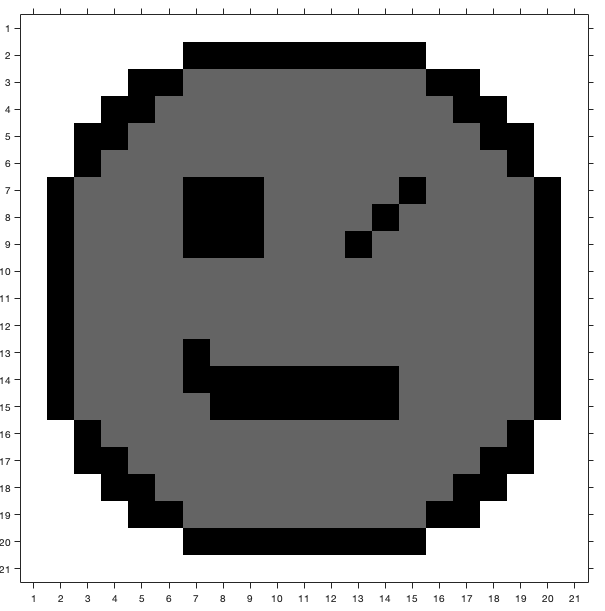
\includegraphics[width=0.6\textwidth]{left_wink.png}
\end{center}

\end{enumerate}

\end{problem}

\begin{problem}
{\bf - Smiley Face Convolutions}

\begin{enumerate}

Now we'll use some common image processing techniques as an opportunity to practice matrix manipulation. We're going to primarily employ what's called a \emph{convolution}.

\item A convolution applies what's called a \emph{kernel} matrix, $K$, to a larger matrix,$A$, and produces a new matrix $K*A$. The kernel matrix is typically small. For instance in all of our examples we're going to use a $3\times 3$ kernel. 

What a convolution does is slide the kernel matrix over the larger matrix $A$, and uses the values of $A$ in the location of the kernel to compute a new value for the output matrix.

In the course live script, if you use the \texttt{smiley\_sliding\_black\_box()} function, you will see a GIF of a kernel sliding over a matrix, like this:

\begin{verbatim}
  A = smiley_wink;
  linalg.smiley_sliding_black_box(A, 2)
\end{verbatim}

%include a centered YouTube video of the sliding black box
\begin{center}
  \youtube{u_8Jc7K_Id4}
\end{center}

As seen in the video, the $3\times 3$ kernel matrix slides over the smiley face matrix. At each instance, the convolution will do three things:
\begin{enumerate}
\item Multiply the kernel matrix by the values of the smiley face matrix in the location of the kernel.
\item Sum the results of the multiplication to get the new value of the output matrix.
\item Place the new value in the output matrix in the location of the kernel.
\end{enumerate}

\item Let's see an example. We're going to use a $3x3$ kernel matrix $K$ defined as

%a 3x3 matrix of 1s, all divided by 9
$$A=\frac{1}{9}\startmat{ccc}
%make the entries 1s
1 & 1 & 1\\
1 & 1 & 1\\
1 & 1 & 1
\stopmat.$$ 

Using this kernel on the smiley face will take the smiley values in the location of the box, add them up, divide by 9, and place the result in the output matrix in the center of the box.

You can see this in the course live script by running the following code, which produces the following GIF:
\begin{verbatim}
  K=1/9*ones(3,3)
  linalg.smiley_sliding_box_with_center(A, Kernel, 2)
\end{verbatim}

%include a centered YouTube video of the sliding box with center
\begin{center}
  \youtube{g5n3P-xW278}
\end{center}

Notice that the center of the sliding box is often a different color than the original pixel in that location. Along the edge of the smiley face, for instance at $smiley(3,7)$ as seen below, the center is a light gray color instead of the original black edge color. Let's see why.

%Make a figure with two images side by side, centered, called conv_example_1 and conv_example_2
\begin{center}
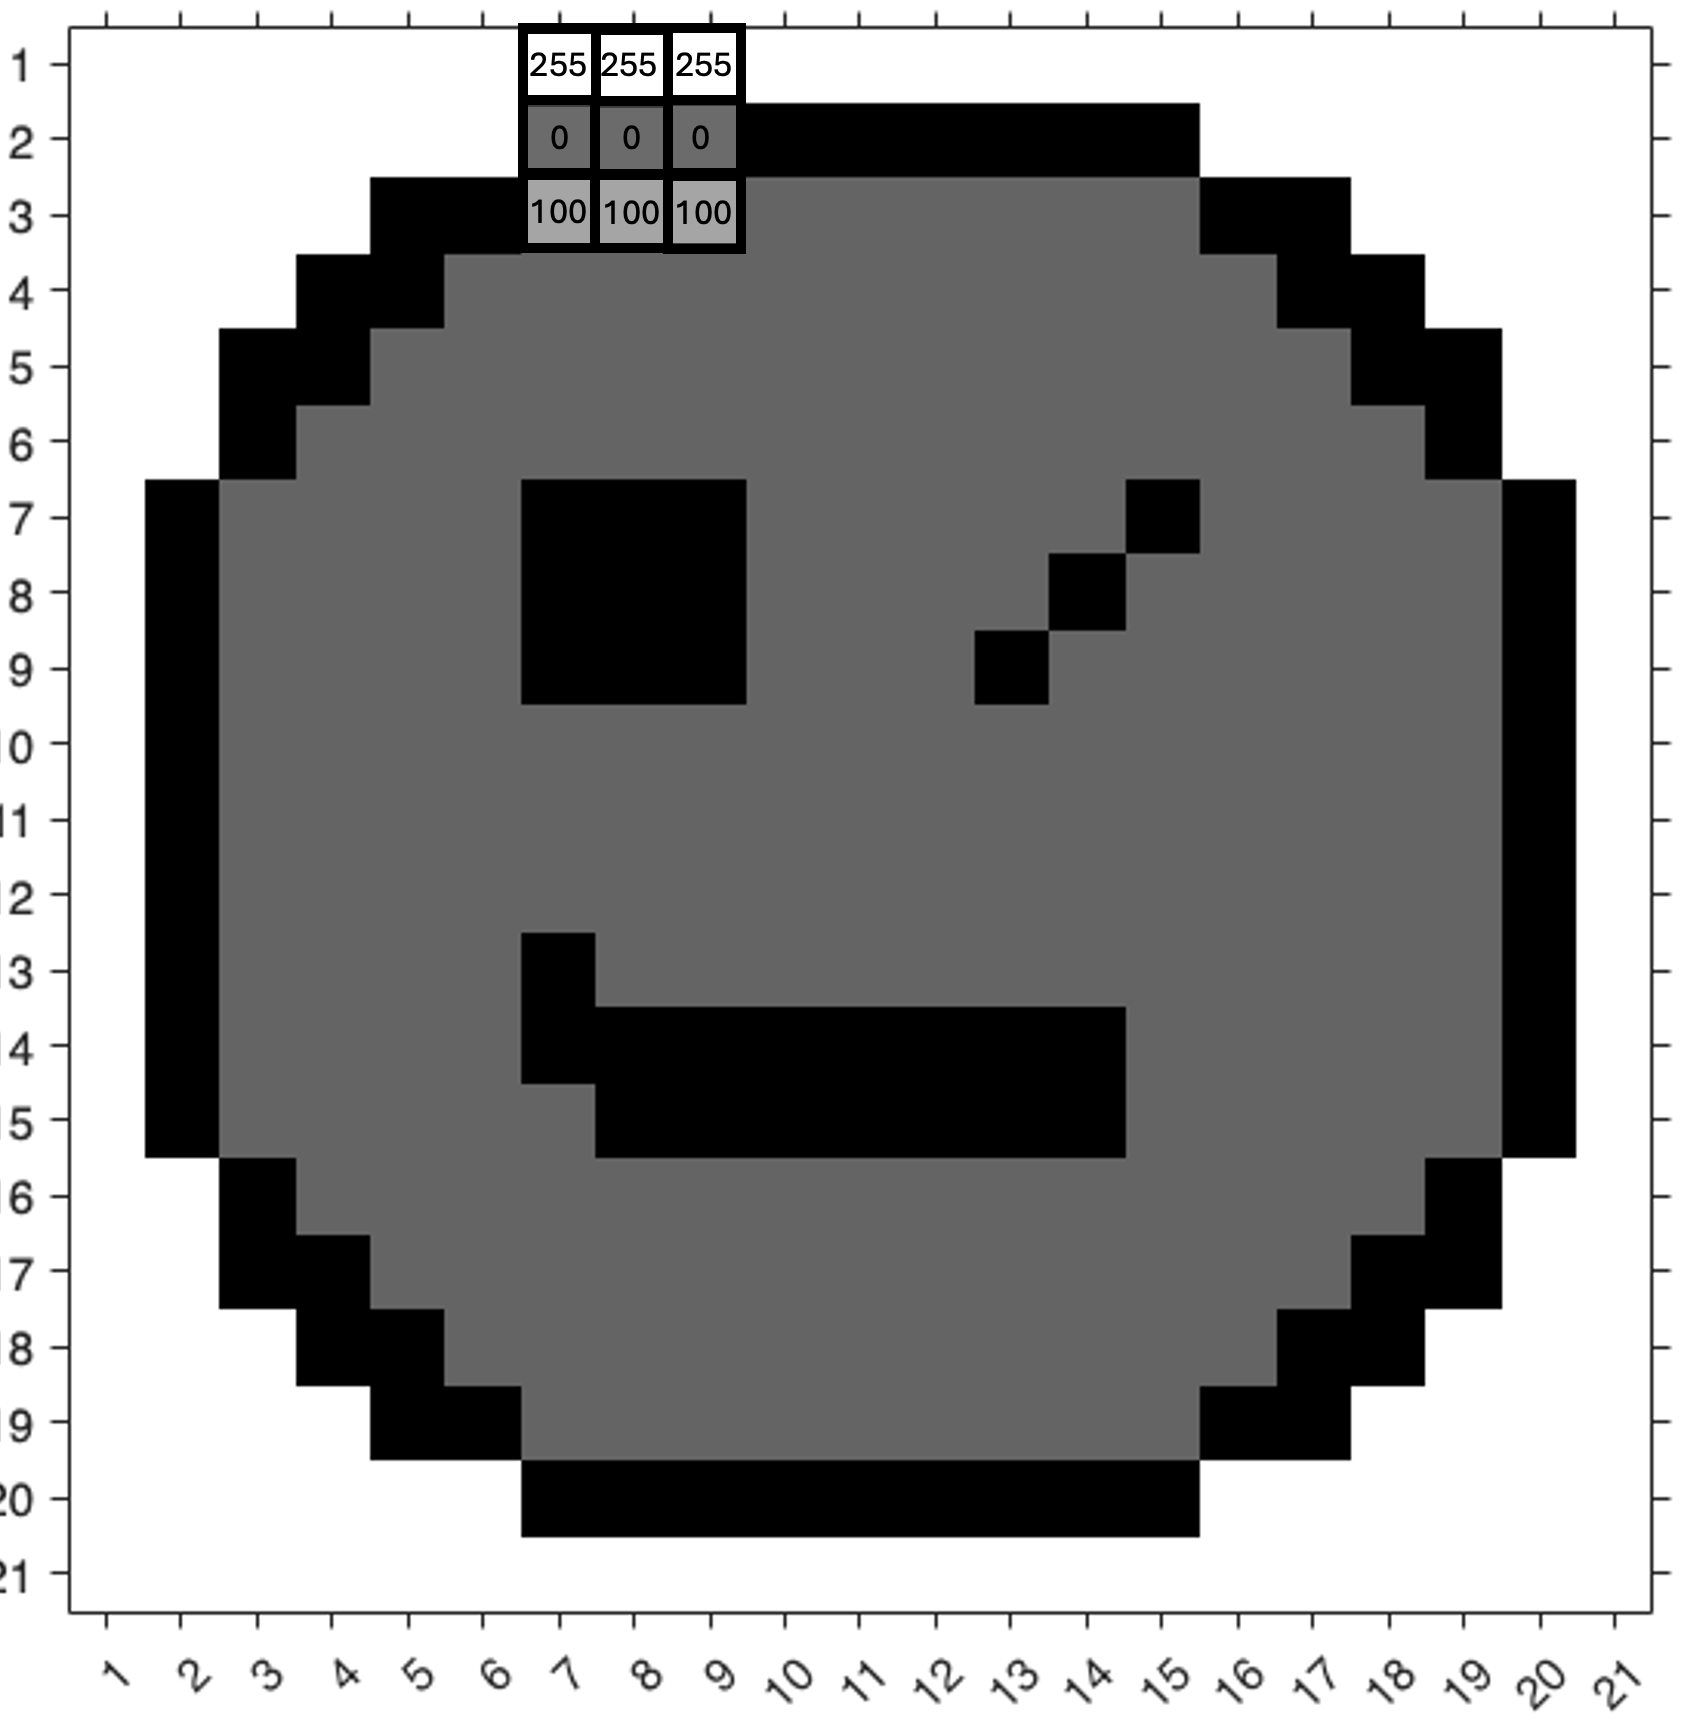
\includegraphics[width=0.45\textwidth]{conv_example_1.png}
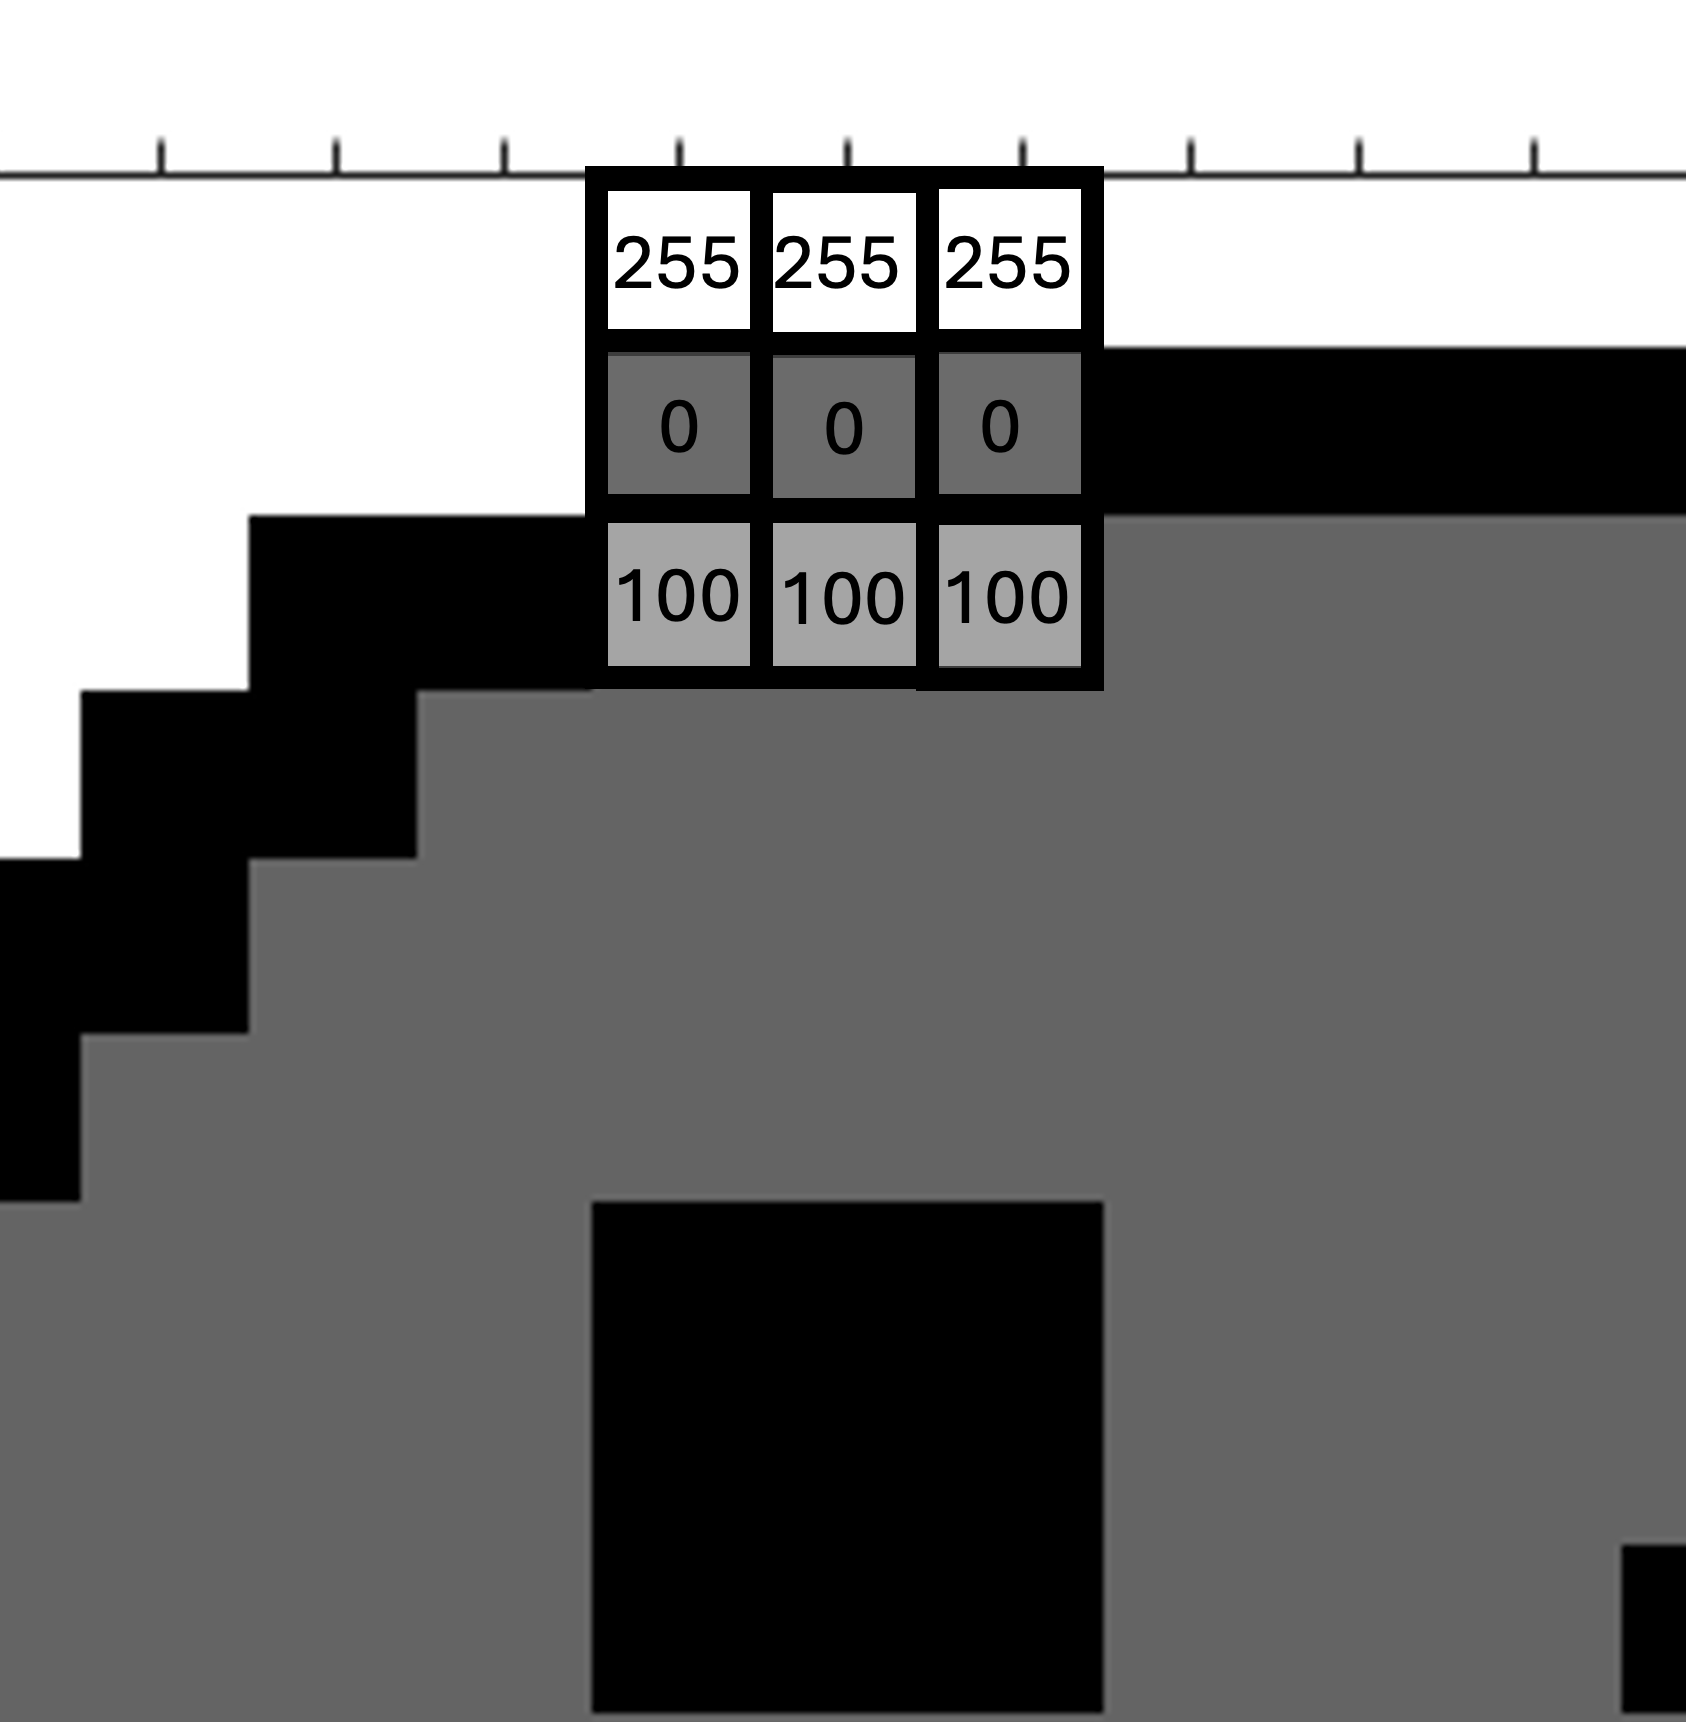
\includegraphics[width=0.45\textwidth]{conv_example_2.png}
\end{center}

The $3\times 3$ grid centered on $smiley(3,7)$ is the sub-matrix
$$\startmat{ccc}
255 & 255 & 255\\
0 & 0 & 0\\
100 & 100 & 100
\stopmat.$$ 

Since the kernel matrix is $A=\frac{1}{9}\startmat{ccc}
1 & 1 & 1\\
1 & 1 & 1\\
1 & 1 & 1
\stopmat$, the convolution will add up $1\cdot 255+1\cdot 255+1\cdot 0+1\cdot 0+1\cdot 0+1\cdot 255+1\cdot 100+1\cdot 100+1\cdot 100$ and divide by $9$ to get around $118.33$. This is why the center of the box is a light gray color instead of the original black edge color.

If we had instead chosen a kernel that more favored the top grid values, the result would be a lighter color instead of a darker color. For instance, if we had chosen the kernel matrix $A=\frac{1}{9}\startmat{ccc}
  2 & 2 & 2\\
  1 & 1 & 1\\
  1 & 1 & 1
  \stopmat$, the convolution be computed as

  $$\frac{1}{9}(2\cdot 255+2\cdot 255+2\cdot 255+1\cdot 0+1\cdot 0+1\cdot 0+1\cdot 100+1\cdot 100+1\cdot 100)\approx 203.33.$$

The convolution does this calculation at every $3\times 3$ grid in the smiley face matrix, and places the result in the center of the grid. This effect is what causes the changes to the smiley face seen below, by running the code below.

\begin{verbatim}
  blurred_face = smiley_wink;
  K=1/9*ones(3,3);
  linalg.smiley_conv_animator(blurred_face,K)
\end{verbatim}

%include a centered YouTube video of the sliding box with center
\begin{center}
  \youtube{E41ETa9MszQ}
\end{center}

You might notice that the effect on the smiley face is a blur. The blur occurs because each pixel is the average of itself and the pixels around it, hence the scalar $\frac{1}{9}$ in the kernel matrix. Kernels will commonly have scalar multiples so that the sum of the kernel is 1.

\item Let's test out the result of some other kernels on different spots of the smiley. If we use the kernel %do a sharpen kernel of -1s except for 9 in the middle
$S=\startmat{ccc}
-1 & -1 & -1\\
-1 & 9 & -1\\
-1 & -1 & -1
\stopmat$, any pixel centered purely on the face (i.e. not touching eyes, smile, or edges) will
\begin{multipleChoice}
  \choice{be slightly lightened.}
  \choice{be vastly darkened.}
  \choice{be vastly lightened.}
  \choice{be slightly darkened.}
  \choice[correct]{remain the same.}
\end{multipleChoice}
This is because the original face color is $100$, while the convolution subtracts $100\cdot\answer{8}$ and adds $100\cdot\answer{9}$, which returns a pixel value of $\answer{100}$.

\item The kernel $S$ gives a \emph{sharpening} effect on the image. Instead of averaging the pixels around the center, it emphasizes the center pixel while de-emphasizing the surrounding pixels, while also not increasing or decreasing the net brightness of the pixel. This is why the center of the face remains the same color.

If we instead look at a face pixel bordering an edge, say $smiley(11,19)$, $S*smiley(11,19)$ (i.e the convolution at that location) will be
\begin{multipleChoice}
  \choice[correct]{white because the edge pixels are zero, overemphasizing the center pixel.}
  \choice{black because the edge pixels are zero, bringing the average down.}
  \choice{the same color because the black and gray pixels cancel out.}
  \choice{light gray because the edge pixels are zero, bringing the average higher.}
\end{multipleChoice}

\item If we wanted to emphasize the sharpening effect, we could increase the value of the center pixel in the kernel.

You will compare the convolutions of the smiley face using the following kernels:

%S0, a weak sharpening kernel with -1/2s and 5 in the middle
$$S_0=\startmat{ccc}
-1/2 & -1/2 & -1/2\\
-1/2 & 5 & -1/2\\
-1/2 & -1/2 & -1/2
\stopmat,$$

%S1, the original sharpening kernel
$$S_1=\startmat{ccc}
-1 & -1 & -1\\
-1 & 9 & -1\\
-1 & -1 & -1
\stopmat,$$

%S2, a strong sharpening kernel with -2s and 17 in the middle
$$S_2=\startmat{ccc}
-2 & -2 & -2\\
-2 & 17 & -2\\
-2 & -2 & -2
\stopmat,$$

and %S3, a very strong kernel with -5s and 41 in the middle
$$S_3=\startmat{ccc}
-5 & -5 & -5\\
-5 & 41 & -5\\
-5 & -5 & -5
\stopmat.$$ 

Use these kernels on the smiley face in the course live script to see the results. First, predict what you think will happen to the smiley face when you use each kernel (i.e. will the sharpening effect continue to increase, will the pixels become more extreme, etc.). Then, run the code below to see the results.

To carry out the convolution, first define the kernel in MATLAB, then use the \texttt{conv2} function to convolve the smiley face with the kernel, then use the \texttt{smiley\_show} function to display the result.

For instance, 

\begin{verbatim}
  Blur = 1/9*[1 1 1; 1 1 1; 1 1 1];
  blurred_face = conv2(smiley_wink, Blur, 'same');
  linalg.smiley_show(S0_face)
\end{verbatim}

\begin{hint}
  The argument \texttt{'same'} in the \texttt{conv2} function tells MATLAB to return a matrix of the same size as the original matrix. This is important because the convolution will shrink the matrix if you don't use this argument.
\end{hint}

Write a reflection on the results. Describe whether you were surprised, why you made your initial guess, and most importantly explain the results you saw mathematically.

\begin{hint}
  The pixel values must range between 0 and 255, so values above 255 will be set to 255 and values below 0 will be set to 0.
\end{hint}

\end{enumerate}

\end{problem}

\section*{Working With Convolutions}

\begin{problem}
{\bf - Image Manipulation}
\begin{enumerate}
  \item Fill in the below $3\times 3$ kernel matrix $K$ to create a kernel that will shift the entire face one step up and to the right.

  %a 3x3 matrix with 0s except for 1 in the bottom right corner, put \answer{} in the entries

  $$K=\startmat{ccc}
  \answer{0} & \answer{0} & \answer{1}\\
  \answer{0} & \answer{0} & \answer{0}\\
  \answer{0} & \answer{0} & \answer{0}
  \stopmat.$$
  
  \item What happens if we keep applying a blur kernel to the smiley face? Make a prediction, then test it out with a for loop in MATLAB and write a reflection on the results.
  
  \begin{hint}

    In MATLAB you can re-define a variable by setting it equal to a new value. If you wanted to keep applying a blur kernel to the smiley face, you can re-define the blur smiley as the convolution of itself with the blur kernel, like this:
    \begin{verbatim}
      blur_smiley = conv2(blur_smiley, Blur, 'same');
    \end{verbatim}

  \end{hint}

\end{enumerate}

\end{problem}

\begin{problem}
{\bf - Working with Bigger Images}

When working with standard images, the matrices can be quite large. 

%SOMETHING SOMEWHERE that requires them to like, add images together, maybe average them, blend them with a moving weight, take the negative, remove just the face of the lion, etc. 

\end{problem}


\end{document}